%%%%%%%%%%%%%%%%%%%%%%%%%%%%%%%%%%%%%%%%%%%%%%%%%%%%%%%%%%%%%%%%%%%
%                                                                 %
%                            CHAPTER TWO                          %
%                                                                 %
%%%%%%%%%%%%%%%%%%%%%%%%%%%%%%%%%%%%%%%%%%%%%%%%%%%%%%%%%%%%%%%%%%%

\chapter{PREVIOUS WORK}
%\resetfootnote %this command starts footnote numbering with 1 again.

The data versioning landscape produces a variety of different approaches and standards towards change capture.
Massive centralized data stores, however, have become more prevalent as data distribution methods advance  \cite{Vassiliadis1999}.
Collection into larger unified repositories will likely require a multi-tiered approach to synchronize the varied practices  \cite{Baker2009}.
Baker notes that differences depend on the sociotechnical distance of a repository from the data's origin \cite{Baker2009}.
Local stores closer to the collection site better understand data capture conditions, but must also adapt to changing environments.
This work provides a basis for understanding the formal underlying properties which will allow consistent versioning practices.
Science agencies and organizations are only beginning to formally codify and standardize methods to capture and publish lineage information \cite{MatthewS.Mayernik201312-039}.
This seems to be a recurring cycle of attention with rapidly developing technologies such as the grid or parallel computing \cite{Kovse2003VGridAVS}.
The CERN grid for the Compact Muon Solenoid experiment carefully developed necessary processes which allow references by multiple users to the same file without copying that file across the grid \cite{Holtman:687353}.

\section{Provenance}

A number of linked data models include versioning concepts such as the Open Provenance Model (OPM) \cite{moreau2008open}.
Driven by the uncertain needs and sometimes conflicting conventions of different scientific domains, the model sought to find a method to standardize the way in which provenance data is captured while also keeping the specification open to accommodate current data sets through the change.
In an experimental case, the model has been applied to sensor networks, automating and unifying their provenance capture even as they grow \cite{5478496}.
To aid OPM's adoption, the framework Karma2 integrates provenance capture into scientific workflows and provides a more abstract view of their data collection activities \cite{simmhan2010karma2}.
The property WasDerivedFrom constitutes a core concept in the model and marks the reliance of one object's existence on another object.
For a large part, this encompasses the engagement which provenance models view versions, without further need to explore the derivation's content.

PROV, a World Wide Web Consortium (W3C) Recommendation, delineates a method to express data provenance in a more compact form as seen in Figure \ref{PROVO} \cite{Gil2013a} \cite{Groth2013}.
The recommendation uses a conceptual model relating activities, agents, and entities to describe data production lineage \cite{Moreau2013c} \cite{Nies2013} \cite{Nies2013a}.
Intended as a high level abstraction, it takes an activity-oriented approach to provenance modeling.
Every data entity results from the actions of some activity.
The conceptual model's expression occurs through the PROV Ontology (PROV-O), which can be conveyed through various resource description languages \cite{Hua2013} \cite{Klyne2013}.
The ontology is further formalized into a functional notation for easier human consumption \cite{Moreau2013b} \cite{Cheney2013a}.
One particular strength that has contributed to the adoption of PROV is its ability to link into other ontologies, making it easier for existing semantically enriched data sets to adopt PROV \cite{Miles2013} \cite{Moreau2013}.
\begin{figure}
	\centering
	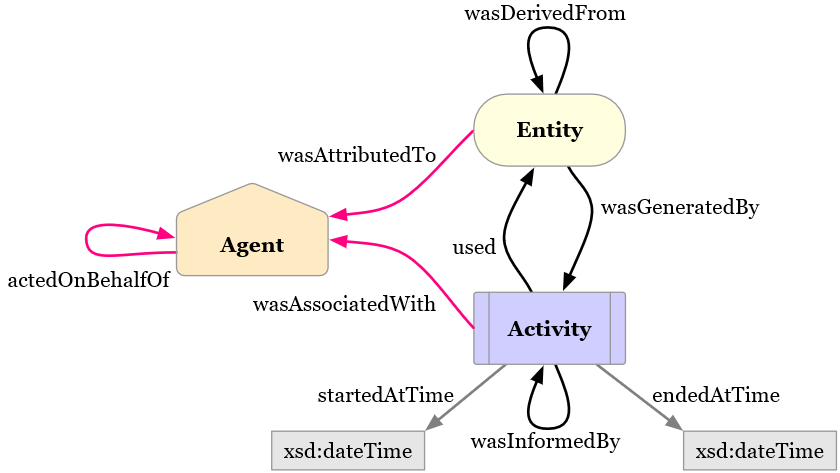
\includegraphics[scale=0.5]{figures/ProvO.png}
	\caption[Diagram of the PROV Ontology.]{Diagram of the PROV Ontology.  Figure 1 from \cite{Lebo2013}}
	\label{PROVO}
\end{figure}
Komadu, a framework developed to alleviate workflow integration, improves upon its predecessor, Karma, by no longer utilizing global context identifiers that were not necessarily shared throughout the workflow. \cite{Suriarachchi_2015}.


The PROV Ontology provides three different concepts that begin to encapsulate the provenance relationship between data versions.
It defines a \textit{prov:Generation} as "the completion of production of a new entity by an activity," \cite{Lebo2013}.
This means that the generation, which corresponds to the version addition operation, must result from a \textit{prov:Activity}.
Activities, however, play a much less active role in versioning since object comparisons instead expose changes.
The property creates a relationship between entities and activities, but such a connection may imply that perturbations in the activity resulted in changing the version.
Changes could also result from modifications in the input data, leading to an entirely new generating activity rather than a modified one.
\textit{Prov:Invalidation} likewise makes a similar connection between activities and entities.
This means that PROV-O does not have the direct means to communicate the addition and invalidation relationships which exist in our versioning context.
Since we previously establish a state-based view between versions, a more contextually appropriate property should connect two objects together.
Continuing, \textit{prov:Derivation} does relate two entities and the ontology defines it as, "a transformation of an entity into another, an update of an entity resulting in a new one, or the construction of a new entity based on a preexisting entity. " \cite{Lebo2013}.
In the Marine Biodiversity Virtual Laboratory (MBVL) dataset's case described in Section \ref{sec:MBVL}, none of these three assertions hold true. 
The process simultaneously considers all four versions so one is not transformed into another as would a sequential set of versions.
Additionally, since we do not know which version is the best, we cannot consider any data set as an update of the others.
Finally, no entity preexisted as the data sets resulted from an ongoing analysis and further steps have not been developed.

The Provenance, Authorship, and Versioning (PAV) Ontology is, "a lightweight vocabulary, for capturing ``just enough” descriptions essential for web resources representing digitized knowledge" \cite{Ciccarese2013}.
It provides a means to track versioning information through linked data by introducing \textit{pav:version} to cite versions and \textit{pav:previousVersion} to link them together in order \cite{Ciccarese2013}.
It does so in comparison to the Dublin Core concept \textit{dc:isVersionOf} which records, "Changes in version imply substantive changes in content rather than differences in format" \cite{DCMI2012}.
PAV supports the idea that a new concept becomes necessary to cover cases where new versions do not have to be substantive but can still be alternate editions of the original object.
While it documents related versions well, PAV does not dive deeper in explaining the circumstances behind version differences.

The Schema.org \textit{schema:UpdateAction} largely reflect the relationships adopted by this work, and are defined as "the act of managing by changing/editing the state of the object" \cite{Schema}.
The remaining subclasses include the \textit{schema:AddAction}, \textit{schema:DeleteAction}, and \textit{schema:UpdateAction}.
The function of these terms is to provide a means to supply searchable web pages with standardized micro-data.
As a result, they orient their properties towards definitions and characterization but do not provide the right structure for a standardized change capture model.

\section{Provenance Distance}

With increasing complexity, data workflows have developed in such a way that even subtle changes have serious implications for other parts of the workflow \cite{TILMES2011548}.
This observation makes change impact difficult to measure, but one insight begins with provenance's role in workflows.
Provenance can give great insight into a data object's future performance such as the  ability to predict disk usage based on the lineage of a data object \cite{dai2014provenance}.
Efforts have also been made to summarize provenance representations to improve consumption \cite{Ainy:2015:ASD:2806416.2806429}.
Changes to the process creating an object signals the development of a new version.
Studying the magnitude of this deviation, therefore, should give some idea into the resulting object's impact.
This idea, known as provenance distance, seeks to determine the impact of changes in provenance on new data versions through measuring graph edit distances.

\begin{figure}
	\centering
	\begin{adjustbox}{addcode={\begin{minipage}{\width}}{
					\caption[Provenance graph of a Level 3 data product, showing the inter-relations between different data products in generating the final product.]{Provenance graph of a Level 3 data product, showing the inter-relations between different data products in generating the final product.  Figure 2 from \cite{TILMES2011548}}\end{minipage}},rotate=90,center}
		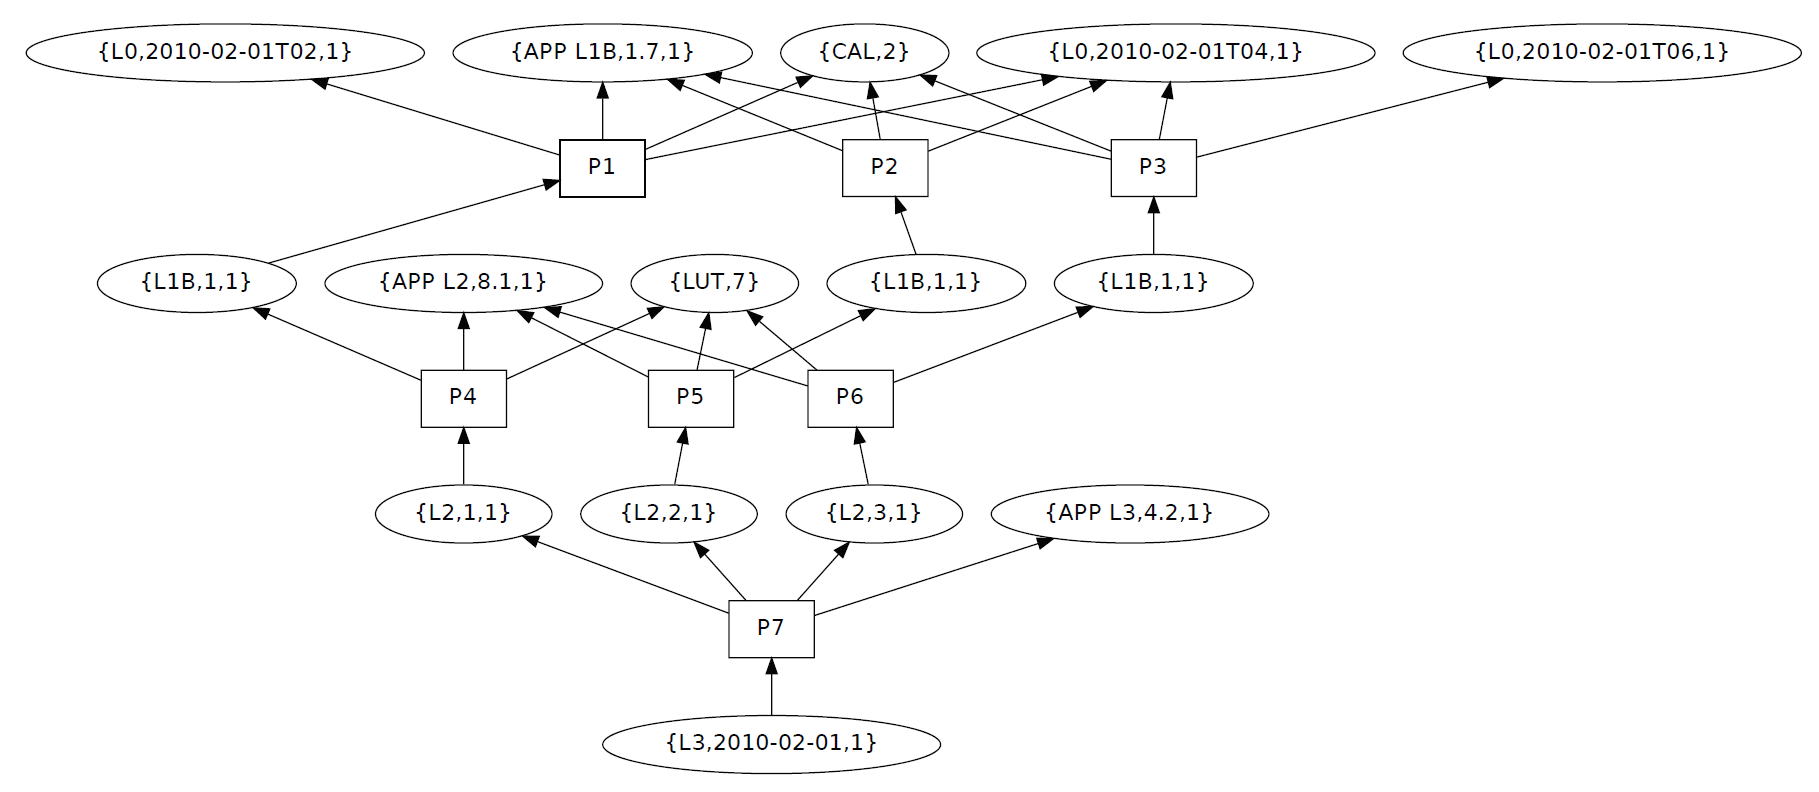
\includegraphics[scale=0.5]{figures/OzoneProvGraph.png}
	\end{adjustbox}
	\label{ProvGraph}
\end{figure}

The first ingredient necessary to calculate provenance distance is a linked data graph capturing the sequence of events leading to the old and new objects' creation, like the one shown in Figure \ref{ProvGraph}.
It shows the multiple lower level products involved in creating a Level 3 ozone indicator.
This can be accomplished through the use of previously mentioned provenance models, but these graphs are not widely available.
Using PROV to represent provenance data in a semantic model produces an acyclic directed graph with labeled nodes.
As a result, the provenance distance problem reduces to similarity measurement.
When calculating this measure, algorithms determine how far two graphs are from being isomorphic \cite{Cao2013}.
Node labeling simplifies this process by providing nodes which must match together, and greatly reduces the complexity from computing generalized graphs.
Graph Edit Distance, counting the edits necessary to transform one graph into another, provides a quantitative measure to associate with this process  \cite{Gao2010}.
Some variations count edge changes \cite{Goddard:1996:DGU:246962.246972}.

In Figure \ref{GraphEdit}, the left graph transforms through a move of edge 1 and a rotation of edge 4, resulting in an edit distance of two.
Such changes in a provenance graph would demonstrate an alteration in dependencies between objects used to generate a final notable product.
This kind of analysis resembles comparison measures employed in determining semantic similarity \cite{Hliaoutakis06informationretrieval}.
Isolating changes responsible for differences in provenance, however, can become difficult in complex environments as Tilmes observes in 2011, 
\begin{quotation}
	Consider the relatively common case of the calibration table, which is an input to the L1B process, changing. Even though the version of the L2 or L3 software hasn't changed, the data files in the whole process have been affected by the change in the calibration.
\end{quotation} \cite{TILMES2011548}.
L-number is shorthand for the level system featured in Figure \ref{NASALevels}.
While provenance distance may be straight-forward to calculate, the indicator hides many insights into an object's behavior.

\begin{figure}
	\centering
	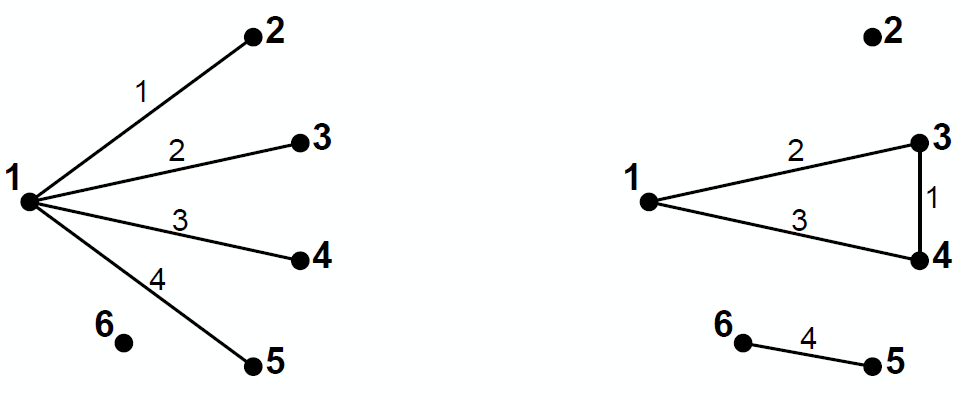
\includegraphics[scale=0.40]{figures/GraphEdit.png}
	\caption[The labeled graph on the left transforms into the right graph under two edge edits.]{The labeled graph on the left transforms into the right graph under two edge edits. Figure 2 from \cite{Goddard:1996:DGU:246962.246972}}
	\label{GraphEdit}
\end{figure}

Methods to provide quality of service boundaries leveraging provenance already exist which compare workflows based on performance criteria \cite{2015:CAA:2778374.2778504}.
These procedures, however, focus primarily on quick retrieval and efficient storage instead of capitalizing on the latent information accessed by reasoning across data set versions \cite{tan2004research}.
The distance measures previously mentioned rely solely on provenance graphs to compute results, but this is obviously insufficient.
When considering the provenance of a data object, methods only consider the activities and entities that took an active role in the production of it.
A new version of an object has a familial relationship with its previous versions, but in most cases, they do not take an active role in its generation.
Without detailed change information, determining the difference between two data objects in a metric beyond broad strokes becomes difficult, if not impossible.

As per our definition of `version', objects must have common provenance, and the more similar they are, the more meaningful the results from versioning methods.
Provenance distance provides a means of determining how reliable versioning results are given a greater adoption of provenance graphs.
Measuring a change's impact with accuracy comparable to a change log requires a more detailed understanding and description than provenance can provide  \cite{Bose:2005:LRS:1057977.1057978}.
Sufficiently precise versioning measurements cannot be provided by provenance distance, but it could indicate the confidence of versioning results, which is out of scope for this project.

\section{Mapping}

Data managers primarily use one of two methods to store data versions: snapshots and deltas.
The snapshot method makes periodic copies of the data's state at a point in time.
While storing and retrieving these snapshots can be very quick, they require significant amounts of space to maintain.
The software manager GIT employs this method and Figure \ref{GITFile} demonstrates an example storage space for multiple versions \cite{Chacon:2009:PG:1618548}.
The squares with dotted outlines indicate unmodified files, which the system stores as pointers instead of full objects.
In addition, GIT compresses and separately stores very old versions which are unlikely to be accessed.
This versioning style may not be ideal for larger or often modified data sets as the size requirements will quickly grow unmanageable.
For many library or catalog environments, they cannot predict, however, the target volume a user desires and must prioritize availability \cite{Payette2002} \cite{Barkstrom_digitallibrary}.
Some methods like the inverted file index have been developed to balance space and retrieval performance on web documents, especially since wikis and news feeds have grown in deployment \cite{Berberich:2007:TMT:1277741.1277831}.
Searches over these text media may require execution on older archived web pages.

\begin{figure}
	\centering
	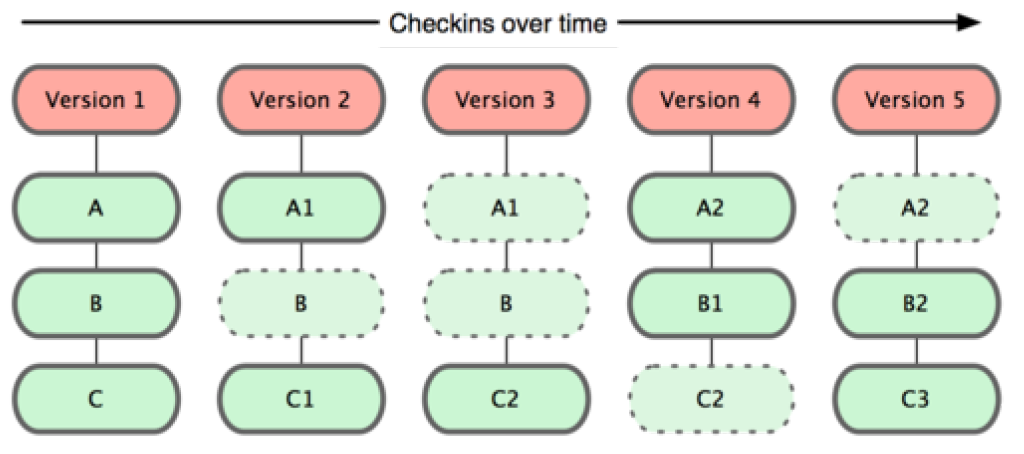
\includegraphics[scale=0.50]{figures/GITFiles.png}
	\caption[GIT stores changes in the repository as snapshots of individual files.]{GIT stores changes in the repository as snapshots of individual files. Figure 1.5 from \cite{Chacon:2009:PG:1618548}}
	\label{GITFile}
\end{figure}

The delta method entails calculating and storing only the differences between one version and the next.
Back delta variations store a snapshot of the most recent version and compute deltas towards older releases.
The forward delta variation stores the oldest data's snapshot and has deltas going forwards.
This method uses the minimum amount of space but trades it in for computation time to recreate any given version.
Particularly long running versioning systems occasionally save an intermittent snapshot to cut down on this processing time.
The setup proves ideal for data sets which prioritize service to their most recent versions \cite{Stuckenholz:2005:CEV:1039174.1039197}.
Because change documentation captures information between version objects, they most resemble differences calculated by the delta method.

Properly detecting changes in a system's files allows file managers to correctly group them into versions as seen in research conducted by the Atmospheric Radiation Measurements (ARM) group \cite{6906868}.
Difference or diff applications must first properly map data between objects and align them for comparison.
Many text-based data sets rely on well-established algorithms to perform this alignment  \cite{Chien:2000:VMX:646544.696357} \cite{Hartung201315}.
Sequential scientific data largely avoids this problem since developers already know the files or objects they replaced.
Users, however, do not have this advantage and system managers are starting to recognize the difference in versioning usage patterns between users and producers \cite{Branco2008}.
Mayernik, et al., probably gives the best description saying, "Prospective records document a process that must be followed to generate a given class of products whereas retrospective records document a process that has already been executed" \cite{MatthewS.Mayernik201312-039}.
While producers take a retrospective approach to version usage, consumers of new versions must take a prospective view, adapting to new changes.
This indicates that the orientation of versioning information reflects the imagined customer of that data.


%%% Local Variables:
%%% mode: latex
%%% TeX-master: t
%%% End:
